\documentclass[12pt]{article}

\usepackage[dvips,letterpaper,margin=0.75in,bottom=0.5in]{geometry}
\usepackage{cite}
\usepackage{slashed}
\usepackage{graphicx}
\usepackage{amsmath}
\usepackage{braket}
\begin{document}


\section{Rattleback}

Tap the rattleback gently downward near one end and the rocking motion you cause will quickly become a spinning motion.  \\ \vskip 0.5cm

\noindent
If you attempt to spin the rattleback in the opposite direction, it will slow down, return to the rocking motion, and begin spinning again in it's preferred direction. \\ \vskip 0.5cm

\noindent
What's going on?  Doesn't this violate conservation of angular momentum?  No!  Friction and the careful asymmetric design of this clever toy conspire to make it appear so!  The toy has three motions, a rolling motion, a rocking motion, and a spinning motion.  For a symmetric object, these motions would all be independent, but not in this case.  When you spin the rattleback in the ``wrong" direction, the spinning motion is translated into a rolling motion, and then a rocking motion, which is then translated into a spinning motion in the opposition direction.\\

To see how these separate motions can be coupled together, consider the cross-section of a rattleback that looks like this:
\begin{center}
{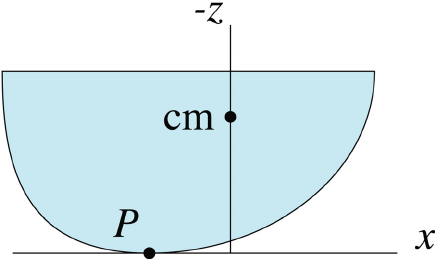
\includegraphics[width=0.40\textwidth]{figs/rattleback_xsec.png}}
\end{center}
The normal force exerted by the table is always upward.  The frictional force is either to the left or to right, depending on which way the toy is spinning.  In one case, the net force points nearly toward the center of mass, and therefore exerts very little torque.  In the other case, the net force points away from the center of mass, exerting a torque that leads to rolling.

\newpage

\section{Antique Motor}

This antique electric motor can be turned on using switching the knife switch.  Please do not touch the large (modern) power supply settings, and please turn off the motor when finished. \\ \vskip 0.5cm

\noindent
Electric motors are a great practical application of the laws of electricity and magnetism:
\begin{center}
{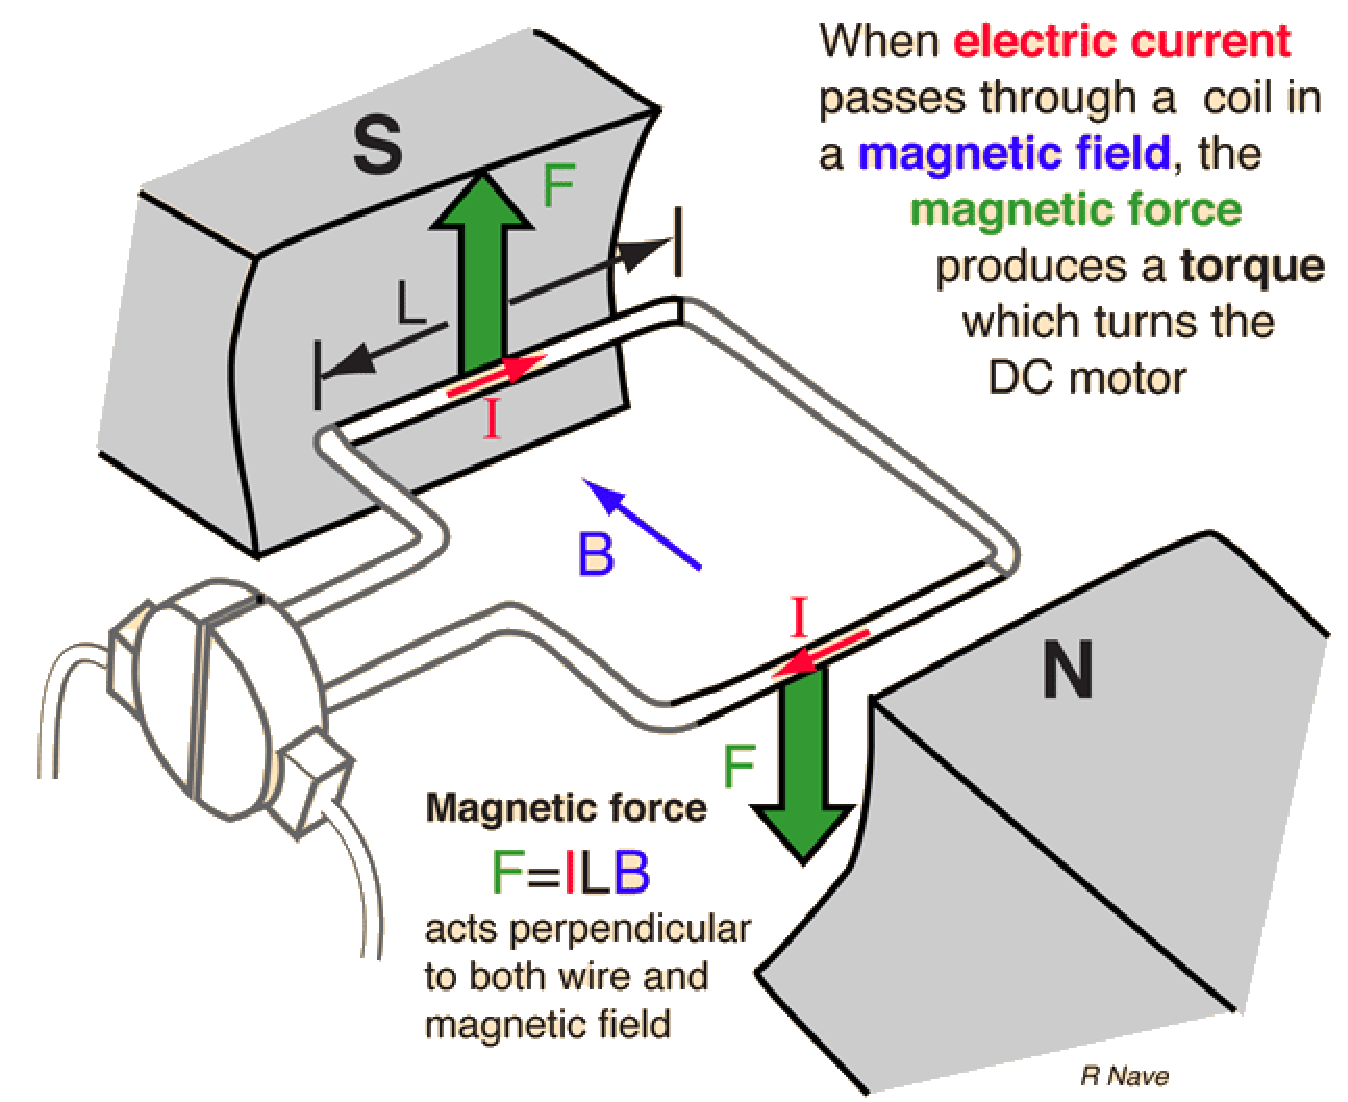
\includegraphics[width=0.80\textwidth]{figs/dcmfor.pdf}}
\end{center}
Practical motors were made possible by combining the understanding of the forces experienced by electric currents in magnetic fields with the clever technical idea of the commutator, which reverses the flow of current through the coil just in time to ensure the torque on the motor is always in the desired direction. \\ \vskip 0.5cm

\noindent
Electricity and magnetism are cornerstones of modern technology.  But the scientist that studied them hundreds of years ago were simply curious to understand the laws of physics related to the curious phenomenon of electricity and magnetism.  They had no idea how useful this technology would be someday.

\newpage


\section{Heat Engine}

All engines work by taking heat energy from a hot reservoir, extracting useful work, and dumping waste heat energy into a cold reservoir.  The waste heat is unavoidable! \\

\noindent
This motor uses a thermoelectric generator based on the Seebeck Effect:
\begin{center}
{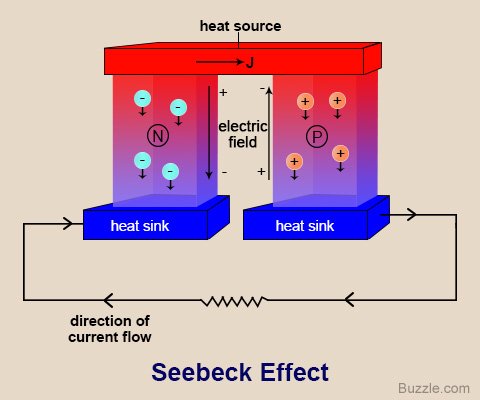
\includegraphics[width=0.80\textwidth]{figs/seebeck.jpg}}
\end{center}
When there's a temperature difference, the mobile charge carriers tend to move away from the hot source faster than they return from the cold source, creating an electric field.  If two dissimilar metals are used, where the mobile charge carriers are positive for one and negative for the other, the fields can line up so that there is a net potential across the whole device, just like a battery.  This energy can be used to power a circuit, in this case, a small motor.

\newpage

\section{What does sound look like?}

In this exhibit you can see what your voice looks like by speaking or whistling into the microphone and watching on the oscilloscope.   \\ \vskip 0.5cm

\noindent
When you speak, you disturb the air, which moves a diaphragm in the microphone, which is designed to produce an electrical signal, which we amplify, and then display on the oscilloscope.  Your voice (or your whistle) should look like a wave because sound is a wave!

\newpage

\section{The Sound of Silence}

With the speakers playing the same tone, you should be able to find places where the noise is substantially reduced.   This is due to destructive interference.

Sound is a wave.  Like all waves, sound can constructively and destructively interfere:
\begin{center}
{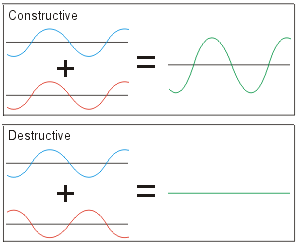
\includegraphics[width=0.80\textwidth]{figs/interference.png}}
\end{center}

The speakers in this exhibit are putting out a single tone of $343~\rm Hz$, which has a wavelength of about one meter.  The back speakers are placed to have about one half of a meter extra distance to your ears, leading to destructive interference.

\newpage

\section{Cloud Chamber}

In this demo you can watch cosmic rays with your own eyes.
\begin{center}
{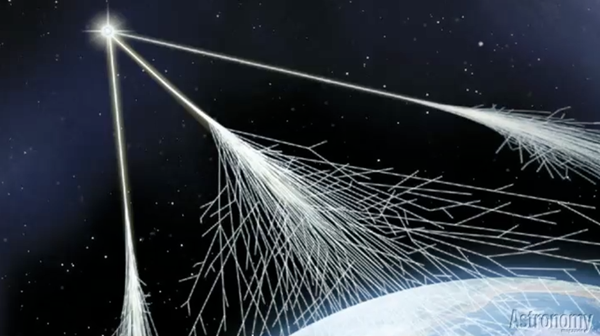
\includegraphics[width=0.80\textwidth]{figs/cosmicrays.png}}
\end{center}
High energy particles from outer space are constantly bombarding our upper atmosphere.  These collisions cause showers of particles, and some of these particles reach us here at surface of the earth.  

Cloud chambers use a supersaturated vapor to charge particles.  When high energy charged particles pass through the gas, they knock electrons off the atoms in the gas creating ions.  These ions act as condensation sites for the supersaturated vapor.  Like rock candy forming on a string in supersaturated sugar water, the cloud condenses around the track of the charged particle, allowing us to see it. 

This cloud chamber uses ethanol chilled by an ice water bath to create the supersaturated vapor layer.

Short fat tracks in chamber are alpha particles, most likely due to background radiation from naturally occurring Radon.

Curly tracks are electrons and positrons.

Long straight tracks are muons.  Muons have a short lifetime, and very few would make it here to the surface of the earth if not for Einsteins theory or special relativity.  So not only are you seeing the effects of particles from outer space, you are also seeing relativity with your own eyes! 

\end{document}




